\chapter{Sperimentazione con Tpot e Darktrace}
\begin{enumerate}
	\item Implementazione di Tpot e analisi dei risultati
	\begin{enumerate}
		\item Configurazione di base
		\item Script e automazioni
		\item Dati raccolti
	\end{enumerate}
	\item Monitoraggio delle reti con Darktrace
	\begin{enumerate}
		\item Definizione e origine degli IDS
		\item Minacce importanti rilevate
		\item Esempi di segnalazioni quotidiane
	\end{enumerate}
	\item Integrare Darktrace e Tpot per una maggiore sicurezza
\end{enumerate}
\section{Implementazione di Tpot e analisi dei risultati}
\subsection{Configurazione di base}
Per prima cosa, è fondamentale verificare di avere tutti i prerequisiti necessari per l'installazione corretta dell'honeypot, questi prerequisiti sono: un indirizzo IP fornito da un server DHCP e una connessione ad Internet, spazio di archiviazione minimo necessario, spazio di memoria RAM. Queste ultime due possono variare in base alla tipologia di installazione \textit{standalone} o \textit{distribuita}. Successivamente, dalla pagina ufficiale Github di T-Pot deve essere scaricata l'immagine ISO; si tratta di un file che contiene l'immagine del sistema operativo preconfigurato con tutti gli strumenti e le funzioni necessarie per T-Pot. Una volta scaricata l'immagine ISO, il passo successivo è l'installazione effettiva dell'immagine. Ciò deve avvenire seguendo attentamente i passaggi indicati fino al completamento dell'installazione, potendo scegliere quale dei tre tipi installare:
\begin{itemize}
	\item \textit{Standalone}: è la versione completa in cui vengono installati tutti i sistemi per far si che funzioni autonomamente.
	\item \textit{Sensor}: è la versione che installa solo il sensore, quindi comprende solo gli honeypot e non i pacchetti per la gestione via interfaccia web.
	\item \textit{Hive}: versione che non include honeypot ma solo programmi per il collegamento ed il controllo da remoto in quanto adibita a raccogliere i dati dalle versioni \textit{sensor}, grazie all'uso di tunnel SSH.
\end{itemize}
Una volta completata l'installazione, viene visualizzato un prompt contenente le informazioni per connettersi al sistema da remoto, questo può essere effettuato tramite l'interfaccia web contenente un terminale oppure tramite connessione SSH. La seguente immagine viene visualizzata in caso T-Pot sia stato installato correttamente ed è pronto all'uso.\\
\begin{center}
	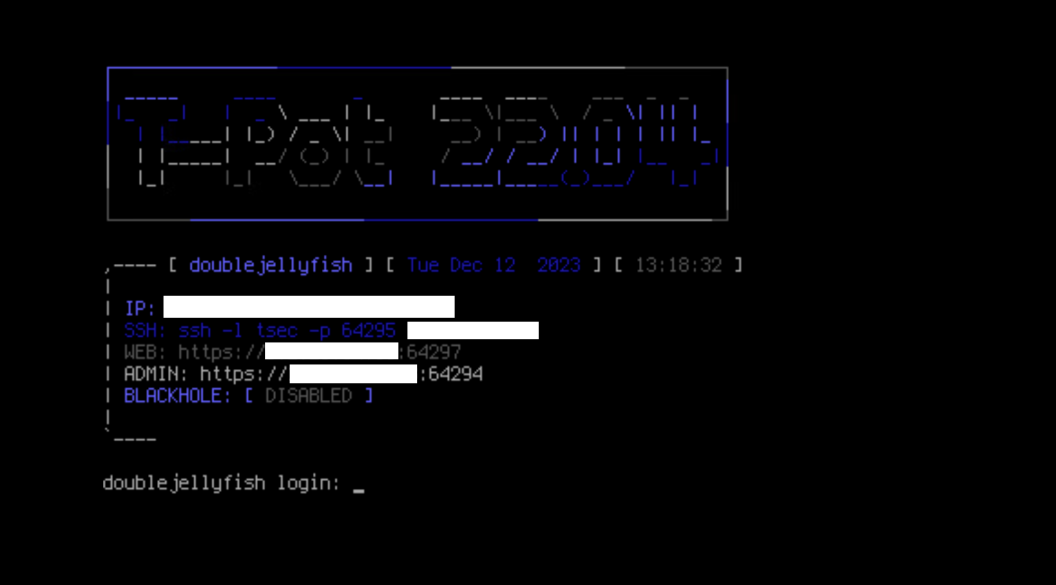
\includegraphics[width=0.8\textwidth]{image/fineInstallazione.png}
\end{center}
Dopo aver completato l'installazione di T-Pot, è necessario apportare alcune modifiche e configurazioni aggiuntive per assicurarsi che funzioni correttamente.\\
Il primo passaggio dopo l'installazione è modificare il file \textit{/etc/network/interface} per configurare correttamente l'interfaccia di rete primaria dell'honeypot. Dopo aver apportato le modifiche al file di configurazione, è necessario riavviare l'interfaccia di rete affinché le modifiche abbiano effetto. Successivamente, è importante installare e configurare il server di posta Postfix utilizzando il gestore di pacchetti apt. Postfix è necessario per consentire a T-Pot di inviare mail contenenti le segnalazioni di connessioni malevole. \\
Durante la configurazione di Postfix, è essenziale assicurarsi che sia configurato per utilizzare la porta 587 per le comunicazioni email anziché la porta standard 25. Ciò è particolarmente importante perché la porta 25 viene occupata dagli Mailoney, mentre la porta 587 offre una maggiore sicurezza.

\subsection{Script e automazioni}
Lo scopo del progetto era di inviare dati degli attacchi subiti da T-Pot al SIEM tramite plugin o programmi esistenti, ma poiché non erano disponibili soluzioni adatte alle esigenze aziendali, è stato sviluppato uno script per analizzare i log dei principali honeypot: 
\begin{itemize}
	\item Dionaea: utilizzato per monitorare la porta legata al protocollo FTP(21).
	\item Cowrie: utilizzato per monitorare le porte legate ai protocolli SSH e Telnet(22, 23).
	\item Tanner: utilizzato per monitorare le porte legate al protocollo HTTP(80, 8080).
	\item Citrixhoneypot: utilizzato per monitorare le porte legate al protocollo HTTPS(443).
	\item Honeytrap: utilizzato per monitorare un gruppo di porte non standard, le porte maggiori di 1024.
\end{itemize}
Lo script estrae le informazioni rilevanti dai log di ogni honeypot e le formatta per l'integrazione con il SIEM.\\
\begin{lstlisting}[language=bash,caption={CEF\_Script.sh}]
#!/bin/bash

honeytrapFile="/data/honeytrap/log/attacker.log"

honeytrapBackup="/home/tsec/script/backup/honeytrap/backup.log"

messaggio=""

if [ ! -e "$honeytrapBackup" ]; then
touch $honeytrapBackup
fi

diffHoneytrap=$(diff $honeytrapFile $honeytrapBackup)
if [ "$diffHoneytrap" != "" ]; then
tmpHoneytrap="/tmp/diffHoneytrap"
diff $honeytrapFile $honeytrapBackup | grep -E '^<|^>' | sed 's/^< //' > $tmpHoneytrap
cp $honeytrapFile $honeytrapBackup
chown tsec:tsec $honeytrapBackup
honeytrapAttaccoPort=$(awk -F'[: ]+' '/^.*tcp/ { print "DeviceName=Honeypot DestinationIP="$11" DestinationPort="$12" ApplicationProtocol= SourceIP="$8" SourcePort="$9"" }' $tmpHoneytrap | sort -u)
if [ ! -z "$honeytrapAttaccoPort" ]; then
messaggio+="Sono state riscontrate le seguenti connessioni alle porte dell'honeypot:\n$honeytrapAttaccoPort\n"
messaggioCEF=$(awk -F'[: ]+' '/^.*tcp/ { print $12" "$8 }' $tmpHoneytrap | sort | uniq -c | awk '{print "reason=Honeytrap cn1="$1" src="$3" dpt="$2}')

echo "$messaggioCEF" | while IFS= read -r linea; do
if [ ! -z "$linea" ]; then
logger -p local4.warn -P 514 -n 127.0.0.1 --rfc3164 -t CEF "0|Honeypot-Test|Honeypot-Test|0.1|event-honeypot-test|end|TRAFFIC|$linea"
fi
done
fi
rm -f $tmpHoneytrap
fi

if [ ! -z "$messaggio" ]; then
echo -e "To: provaAlertEmailMatteo@gmail.com\nSubject: Connessioni all'honeypot\n$messaggio" >> /tmp/mailTemp.txt
/usr/sbin/sendmail provaAlertEmailMatteo@gmail.com < /tmp/mailTemp.txt
rm -f /tmp/mailTemp.txt
fi
\end{lstlisting}
Ecco una spiegazione delle principali azioni svolte dallo script:
\begin{enumerate}
	\item Viene definito il percorso del file di log dell'honeypot e il percorso del file di backup che conterrà una copia del file di log per confronti successivi.
	\item Se il file di backup non esiste, viene creato.
	\item Viene eseguito un confronto tra il file di log attuale e quello di backup per individuare eventuali differenze.
	\item Se vengono rilevate delle differenze, vengono estratte le informazioni sulle connessioni di attacco dal file di log attuale.
	\item Queste informazioni vengono aggiunte a un messaggio di notifica che sarà inviato tramite email.
	\item Viene generato un messaggio nel formato CEF (Common Event Format) per ciascuna connessione di attacco trovata.
	\item Infine, se è stato creato un messaggio di notifica, viene creato un file temporaneo contenente il testo dell'email di notifica e viene inviata l'email utilizzando il comando sendmail.
\end{enumerate}
Questo processo viene effettuato per i cinque honeypot elencati precedentemente. Per far sì che lo script esegua il controllo dei log ogni minuto, è necessario configurare il file crontab. Questo file è collegato al comando crontab, il quale, all'avvio del sistema, esegue un demone che legge il file ogni minuto.\\
Successivamente, è necessario creare un altro script che permetta la cancellazione delle cartelle di backup utilizzate per il confronto all'avvio del sistema, al fine di mantenere la logica del programma integra.

\clearpage

\begin{lstlisting}[language=bash,caption={Delete\_Script.sh}]
#!/bin/bash

# Specifica i percorsi dei file che vuoi cancellare
dionaeaBackup="/home/tsec/script/backup/dionaea/backup.json"
cowrieBackup="/home/tsec/script/backup/cowrie/backup.json"
tannerBackup="/home/tsec/script/backup/tanner/backup.json"
citrixhoneypotBackup="/home/tsec/script/backup/citrixhoneypot/backup.log"
honeytrapBackup="/home/tsec/script/backup/honeytrap/backup.log"

# Cancella i file
rm -f $dionaeaBackup $cowrieBackup $tannerBackup
rm -f $citrixhoneypotBackup $honeytrapBackup

# Aggiungi altre operazioni di pulizia, se necessario
echo "File cancellati con successo."
\end{lstlisting}
Una volta creato quest'ultimo script, è necessario creare un servizio che esegua quest'ultimo script ad ogni avvio della macchina. Questo può essere fatto utilizzando i servizi di systemctl con il seguente codice:
\begin{lstlisting}[caption={Delete\_Backup.service}]
	[Unit]
	Description=Script per cancellare file prima del riavvio
	
	[Service]
	Type=oneshot
	ExecStart=/usr/local/bin/delete_backup.sh
	
	[Install]
	WantedBy=multi-user.target
\end{lstlisting}

\subsection{Dati raccolti}
I dati qui mostrati riguardano tutti gli attacchi subiti dall'honeypot, non solo quelli raccolti dallo script, nell'arco temporale di una settimana in cui T-Pot è stato esposto a Internet.\\
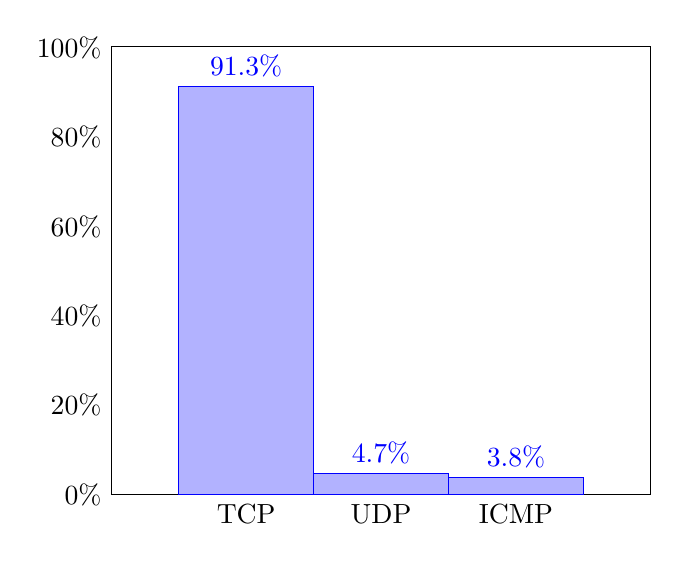
\begin{tikzpicture}
	\begin{axis}[ybar,
		bar width=1,
		ymin=0,
		enlarge x limits={abs=1},
		xtick=data,
		point meta=y*100,
		nodes near coords={\pgfmathprintnumber\pgfplotspointmeta\%},
		nodes near coords style={/pgf/number format/precision=3,
			/pgf/number format/fixed},
		xticklabels={TCP,UDP,ICMP},
		yticklabel={\pgfmathparse{\tick*100}\pgfmathprintnumber{\pgfmathresult}\%},
		tickwidth=0,
		]
		
		\addplot table[x expr=\coordindex,y index=0,row sep=\\] {0.913\\0.047\\0.038\\};
	\end{axis}
\end{tikzpicture}\\
L'analisi dei dati raccolti rivela che la quasi totalità dei pacchetti ricevuti è di tipo TCP, rappresentando il 91,3\% del totale, seguito da UDP con il 4,7\% e ICMP con il 3,8\%. Questo è in linea con il fatto che il protocollo TCP richiede un maggior numero di pacchetti per la sua affidabilità.\\
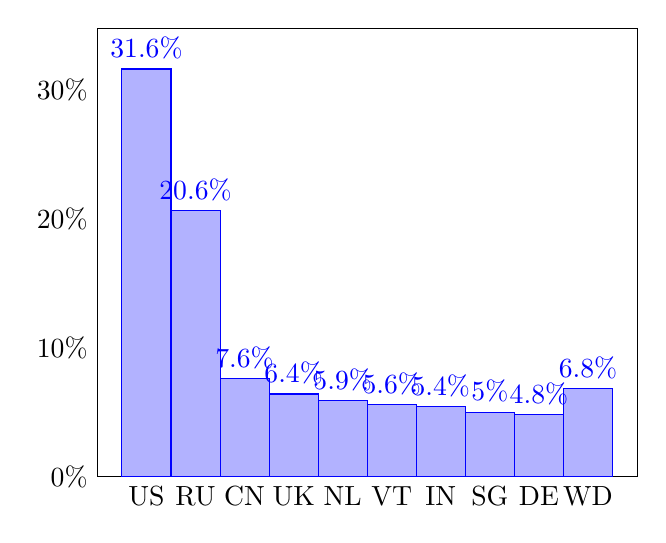
\begin{tikzpicture}
	\begin{axis}[ybar,
		bar width=1,
		ymin=0,
		enlarge x limits={abs=1},
		xtick=data,
		point meta=y*100,
		nodes near coords={\pgfmathprintnumber\pgfplotspointmeta\%},
		nodes near coords style={/pgf/number format/precision=2,
			/pgf/number format/fixed},
		xticklabels={US,RU,CN,UK,NL,VT,IN,SG,DE,WD},
		yticklabel={\pgfmathparse{\tick*100}\pgfmathprintnumber{\pgfmathresult}\%},
		tickwidth=0,
		]
		
		\addplot table[x expr=\coordindex,y index=0,row sep=\\] {0.316\\0.206\\0.076\\0.064\\0.059\\0.056\\0.054\\0.050\\0.048\\0.068\\};
	\end{axis}
\end{tikzpicture}\\
Mentre dal punto di vista geografico, gli Stati Uniti d'America, la Russia e la Repubblica Popolare Cinese sono i principali attori; infatti, contribuiscono complessivamente al 59,8\% di tutti gli attacchi registrati, seguiti da altri paesi come Regno Uniti, Paesi Bassi, Vietnam, India, Singapore, Germania e il resto del mondo, che rappresenta il 6,8\%.\\
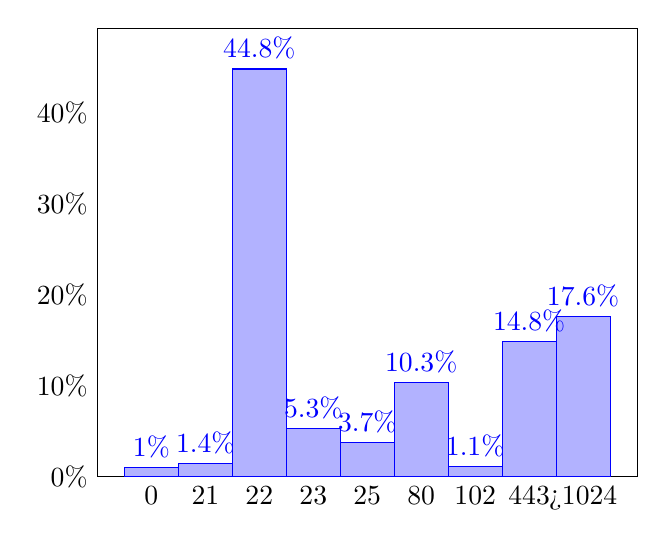
\begin{tikzpicture}
	\begin{axis}[ybar,
		bar width=1,
		ymin=0,
		enlarge x limits={abs=1},
		xtick=data,
		point meta=y*100,
		nodes near coords={\pgfmathprintnumber\pgfplotspointmeta\%},
		nodes near coords style={/pgf/number format/precision=3,
			/pgf/number format/fixed},
		xticklabels={0,21,22,23,25,80,102,443,>1024},
		yticklabel={\pgfmathparse{\tick*100}\pgfmathprintnumber{\pgfmathresult}\%},
		tickwidth=0,
		]
		
		\addplot table[x expr=\coordindex,y index=0,row sep=\\] {0.010\\0.014\\0.448\\0.053\\0.037\\0.103\\0.011\\0.148\\0.176\\};
	\end{axis}
\end{tikzpicture}\\
Nel dettaglio delle porte più attaccate, la porta 22 (SSH) risulta essere quella bersagliata più frequentemente, il 44,8\% di tutti gli attacchi diretti sono a questa porta. Le porte 443 (HTTPS) e 80 (HTTP) seguono rispettivamente con il 14,8\% e il 10,3\%. Altre porte di rilevanza includono la porta 23 (Telnet) e la porta 25 (SMTP), mentre le porte non standard, quelle non standard ($>$1024), contribuiscono in misura minore agli attacchi subiti.

\section{Monitoraggio delle reti con Darktrace}
\subsection{Minacce importanti rilevate}
Nel contesto di questa sezione, saranno esaminati tre casi di anomalie rilevate e risolte utilizzando Darktrace.\\
Il primo caso riguarda il worm Conficker (CVE-2008-4250), scoperto nel 2008, che sfrutta una vulnerabilità non ancora corretta di Microsoft Windows, al fine di violare la password di amministratore locale. Una volta ottenuto il controllo di un dispositivo, il worm cerca di diffondersi ad altre macchine nella rete. Darktrace ha riconosciuto questa minaccia tramite il rilevamento di grandi richieste DNS domini generati da algoritmi (DGA). Di fronte a tale minaccia, Darktrace ha messo automaticamente il dispositivo interessato in quarantena, rimuovendolo dalla rete fino a quando un operatore umano non ha deciso di rilasciarlo.\\
La seconda anomalia significativa coinvolge l'uso di strumenti di attacco e ricognizione, come Nmap, Nessus o OpenVAS, da parte di un dispositivo di rete per condurre scansioni e catalogare informazioni su indirizzi IP, porte aperte, sistemi operativi e vulnerabilità. Darktrace ha riconosciuto quante e quali porte/servizi sono stati scansionati ed è intervenuto bloccando tutte le connessioni in uscita del dispositivo coinvolto. L'analista responsabile ha poi contattato il cliente per informarlo sull'attività sospetta all'interno della sua rete.\\
Infine, nel terzo caso, Darktrace ha rilevato un'anomalia denominata "Ransomware / SMB Reads then Writes with Additional Extensions". In questo scenario, è stato osservato un dispositivo che ha letto un gran numero di file SMB con un'estensione specifica, seguito dalla scrittura di un numero corrispondente di file con un'estensione aggiuntiva. Questo comportamento poteva essere indicativo di un attacco ransomware. Darktrace ha consigliato di esaminare attentamente i file scritti per verificare se corrispondessero a un'estensione tipica dei ransomware.

\subsection{Esempi di segnalazioni quotidiane}
Le segnalazioni quotidiane possono essere suddivise in due categorie: comune e media gravità. Tra gli incidenti comuni segnalati quotidianamente troviamo:
\begin{itemize}
	\item \texttt{Plaintext password}: questo tipo di segnalazione indica l'individuazione di login inviati in chiaro, ovvero senza alcuna cifratura delle credenziali. Questi eventi possono verificarsi nei protocolli HTTP o LDAP. I login scoperti vengono successivamente inclusi nel report settimanale inviato all'azienda.
	\item \texttt{Possible Unencrypted Password File On Server}: questo incidente si verifica quando un dispositivo apre un documento con nel titolo le parole "password", "pwd" o "secret", e non utilizza un formato noto per la sicurezza, ma un formato comune come .doc o .xlsx. Tali file vengono segnalati nel report settimanale.
	\item \texttt{Anonymous NTLM logins}: questa segnalazione avviene quando un dispositivo tenta di autenticarsi con altri dispositivi tramite NTLM utilizzando un account utente anonimo. Questi tentativi di login anonimi vengono poi inclusi nel report settimanale consegnato al cliente.
\end{itemize}
Le segnalazioni di media gravità, che richiedono un'analisi più approfondita, includono:
\begin{itemize}
	\item \texttt{Suspicious Domain}: questo tipo di segnalazione avviene quando un dispositivo si connette a un dominio esterno raro, non comunemente visitato all'interno della rete, con un dominio di primo livello (TLD) associato ad attività dannose, come ad esempio "example.top". Il compito dell'analista è verificare la legittimità del sito, utilizzando strumenti come Cisco Talos o VirusTotal.
	\item \texttt{Unusual Admin RDP Session}: questa segnalazione si verifica quando viene effettuata una connessione RDP (Remote Desktop Protocol) con credenziali di amministratore. L'analista contatta solitamente il cliente per verificare la legittimità dell'operazione.
	\item \texttt{BitTorrent}: viene segnalato quando un dispositivo stabilisce connessioni peer-to-peer BitTorrent, spesso associato alla condivisione di dati protetti da copyright o ad altre informazioni indesiderate. In questo caso, si consiglia al cliente di indagare sulla quantità di dati scaricati e di disinstallare il programma dai dispositivi aziendali.
\end{itemize}

\section{Integrare Darktrace e Tpot per una maggiore sicurezza}
L'integrazione di Darktrace e T-Pot offre una serie di vantaggi significativi per la sicurezza informatica. Da un lato, Darktrace con la sua capacità di rilevare e prevenire intrusioni in tempo reale, consente di identificare e rispondere prontamente alle minacce attive. Tuttavia, può essere limitato dalla sua capacità di rilevare solo le minacce già note o le firme di attacco conosciute. D'altro, T-Pot agisce come esca per attirare gli attaccanti e raccogliere informazioni sulle loro tattiche e strategie. Integrando questi due strumenti, è possibile prevenire gli attacchi esterni, i quali vengono attratti e intrappolati da T-Pot; contemporaneamente è possibile bloccare gli attacchi che si verificano all'interno della rete, migliorando così complessivamente la sicurezza dell'ambiente informatico.